\begin{center}
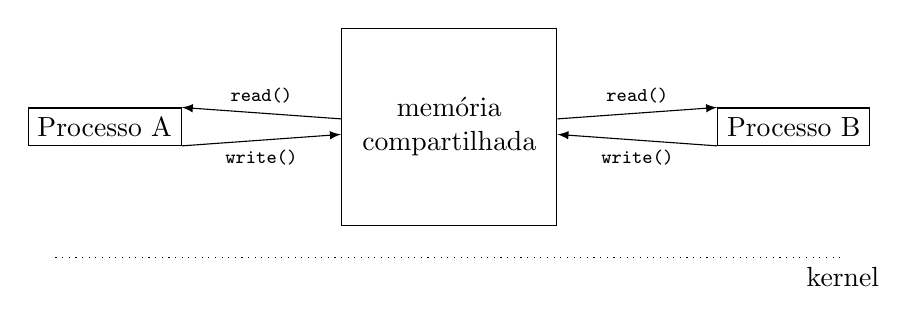
\begin{tikzpicture}
\def\shift{2.5cm}
\def\yshift{\shift/1.5}
\tikzset{base/.style={draw},
mem/.style={base,minimum width=\shift,minimum height=\shift,align=center},
proc/.style={base},
every path/.style={>=latex,draw},syscal/.style={font=\scriptsize\tt}}
\node[mem,text width=\shift] at (0,0) (MEM) {memória\\ compartilhada};
\node[proc] at (-1.75*\shift,0) (PA) {Processo A};
\node[proc] at (1.75*\shift,0) (PB) {Processo B};
\path[->] (PA.south east) -- node[syscal,below]{write()} (MEM);
\path[->] (MEM) -- node[syscal,above]{read()} (PA.north east);
\path[->] (MEM) -- node[syscal,above]{read()} (PB.north west);
\path[->] (PB.south west) -- node[syscal,below]{write()} (MEM);
\draw[dotted] (-2*\shift,-\yshift) -- (2*\shift,-\yshift) node[below] {kernel};
\end{tikzpicture}
\end{center}
